\documentclass[aspectratio=169]{beamer}
% \usetheme{Madrid}

\usefonttheme{serif}
\setbeamercolor{normal text}{fg=black}

% Make all structural text black (titles, sections, etc.)
\setbeamercolor{structure}{fg=black}

% Frame titles (top title)
\setbeamercolor{frametitle}{fg=black}

% Figure caption ("Figure:")
\setbeamercolor{caption name}{fg=black}
\setbeamercolor{caption}{fg=black}

% Section titles in footer/header
\setbeamercolor{section in head/foot}{fg=black}

% Just in case
\setbeamercolor{title}{fg=black}


% --- Theme setup (minimal) ---
\usetheme{default}
\useoutertheme{default}
\useinnertheme{default}

% Remove navigation symbols
\setbeamertemplate{navigation symbols}{}

% Define your red
% \definecolor{myred}{RGB}{225,120,120}
\definecolor{myred}{RGB}{115,0,10}


\usepackage{color} % color added for editing
\newcommand{\bl}[1]{\textcolor[rgb]{0.00,0.00,1.00}{#1}}
\newcommand{\gr}[1]{\textcolor[rgb]{0.00,0.50,0.00}{#1}}
\newcommand{\rd}[1]{\textcolor[rgb]{0.75,0.00,0.00}{#1}}
\newcommand{\tl}[1]{\textcolor[rgb]{0,0.6,0.60}{#1}}

\usepackage{booktabs}
\usepackage{bm}
\usepackage{mdframed}
\usepackage{xcolor}

% --- Custom footline ---
\setbeamertemplate{footline}{
\leavevmode

% Thin red line (moved to TOP)
\begin{beamercolorbox}[wd=\paperwidth,ht=0.1ex]{}
\color{myred}\rule{\paperwidth}{0.1ex}
\end{beamercolorbox}

\hbox{
\begin{beamercolorbox}[wd=\paperwidth,ht=2.5ex,dp=1ex]{}
\hspace{1em}
\insertsection
\hfill
\insertframenumber{} / \inserttotalframenumber
\hspace{1em}
\end{beamercolorbox}
}
}

% Remove headline entirely
\setbeamertemplate{headline}{}

% Optional: clean fonts
\setbeamerfont{footline}{size=\small}







\title{Chapter~3~Machine Learning Workflows}
\author{Austin R.J. Downey}
\date{}

\begin{document}

\section{Machine Learning for Engineering Problem Solving}
\frame{\titlepage}


\section{Chapter~3~Machine Learning Workflows}



%------------------------------------------------

\section{2.5~Training and Testing Data}

\begin{frame}{Overfitting}
	
	Training and testing on the same dataset is a major mistake.
	
	\vspace{0.5em}
	
	\begin{itemize}
		\item The model can memorize the training data
		\item Training accuracy may appear perfect
		\item Performance on new data may be poor
	\end{itemize}
	
	\vspace{0.5em}
	
	This problem is called:
	
	\[
	\textbf{Overfitting}
	\]
	
	\vspace{0.5em}
	
	Goal:
	\begin{itemize}
		\item Build models that generalize to unseen data
	\end{itemize}
	
\end{frame}

%------------------------------------------------

\begin{frame}{Training and Testing Sets}
	\begin{columns}
		
		\column{0.48\textwidth}
		
		Standard supervised learning workflow:
		
		\vspace{0.5em}
		
		\begin{itemize}
			\item Train model using training data
			\item Evaluate model using test data
			\item Test data must remain unseen during training
		\end{itemize}
		
		\vspace{0.5em}
		
		Notation:
		
		\[
		\mathbf{X}_{\text{train}},
		\quad
		\mathbf{y}_{\text{train}}
		\]
		
		\[
		\mathbf{X}_{\text{test}},
		\quad
		\mathbf{y}_{\text{test}}
		\]
		
		\column{0.52\textwidth}
		\centering
		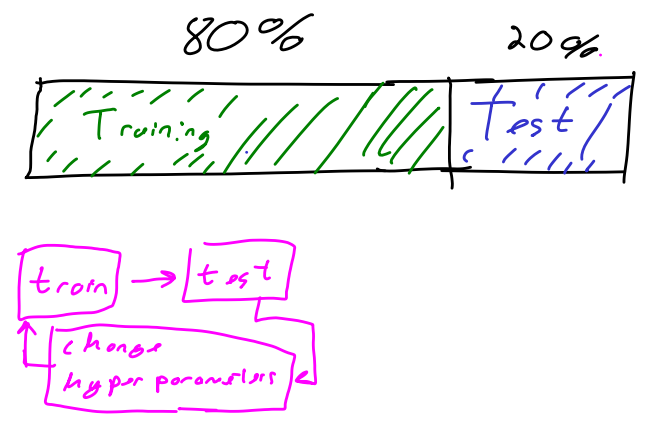
\includegraphics[width=\textwidth]{../figures/training_test_datasets}
		
		\vspace{0.3em}
		{\small Training/testing split.}
		
	\end{columns}
\end{frame}

%------------------------------------------------

\begin{frame}{Validation Sets}
	\begin{columns}
		
		\column{0.48\textwidth}
		
		A validation set is often added to tune models.
		
		\vspace{0.5em}
		
		\begin{itemize}
			\item Training set:
			\begin{itemize}
				\item Learn model parameters
			\end{itemize}
			
			\vspace{0.3em}
			
			\item Validation set:
			\begin{itemize}
				\item Tune hyperparameters
			\end{itemize}
			
			\vspace{0.3em}
			
			\item Test set:
			\begin{itemize}
				\item Final evaluation
			\end{itemize}
		\end{itemize}
		
		\vspace{0.5em}
		
		Scikit-Learn:
		
		\[
		\texttt{train\_test\_split}
		\]
		
		\column{0.52\textwidth}
		\centering
		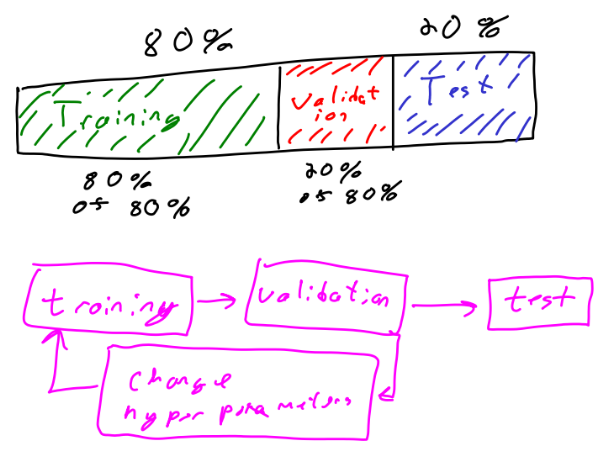
\includegraphics[width=\textwidth]{../figures/training_validation_test_datasets}
		
		\vspace{0.3em}
		{\small Training, validation, and testing workflow.}
		
	\end{columns}
\end{frame}

%------------------------------------------------

\section{2.6~Pipelines}


\begin{frame}{Machine Learning Pipelines}
	\begin{columns}
		
		\column{0.48\textwidth}
		
		Scikit-Learn pipelines combine multiple processing steps into a single workflow.
		
		\vspace{0.5em}
		
		Typical steps:
		\begin{itemize}
			\item Data preprocessing
			\item Feature scaling
			\item Feature engineering
			\item Model training
		\end{itemize}
		
		\vspace{0.5em}
		
		Benefits:
		\begin{itemize}
			\item Cleaner code
			\item Consistent preprocessing
			\item Easier cross-validation
			\item Simplified hyperparameter tuning
		\end{itemize}
		
		\column{0.52\textwidth}
		\centering
		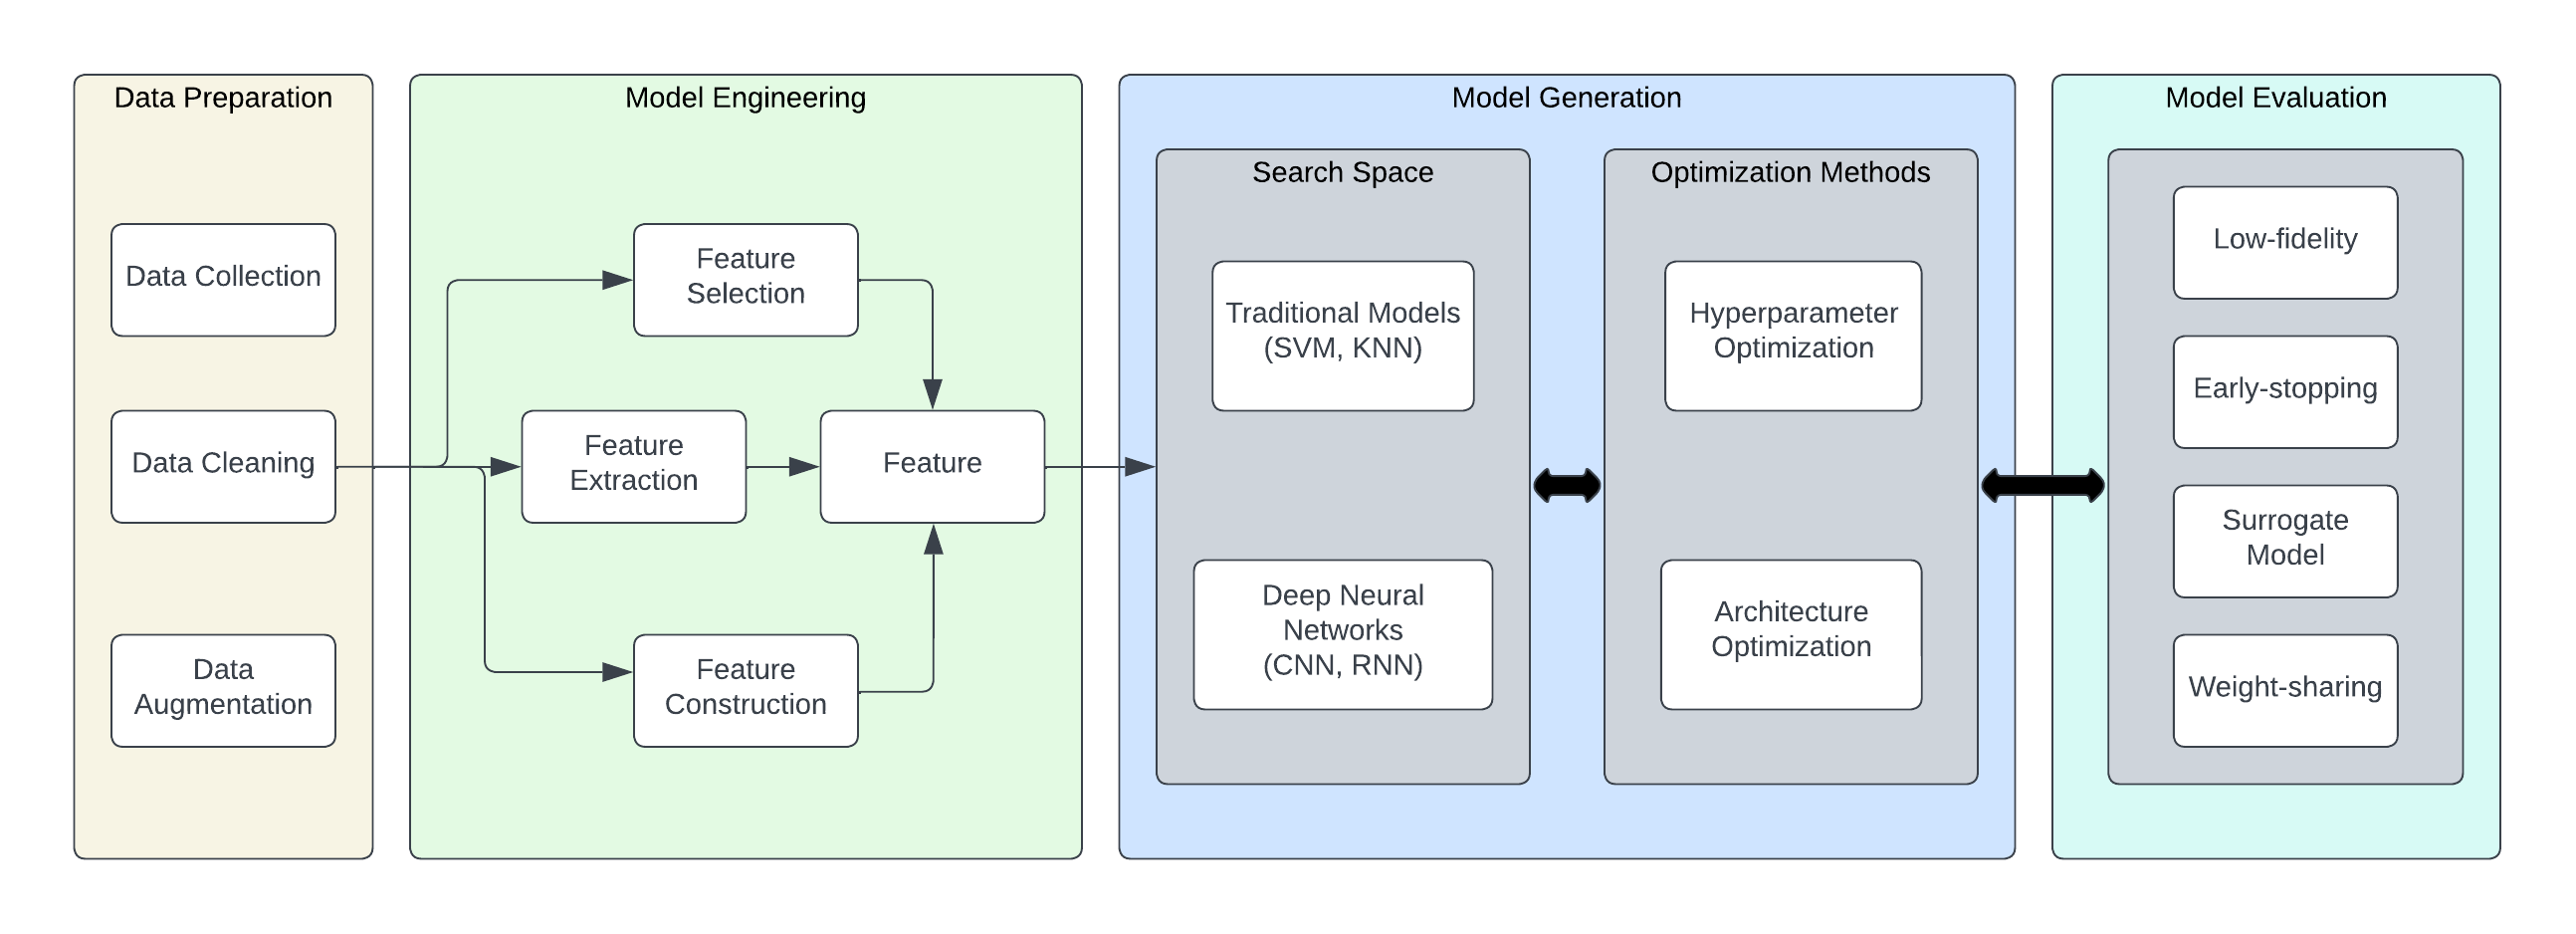
\includegraphics[width=\textwidth]{../figures/AutoML_diagram}
		
		\vspace{0.3em}
		{\small Example machine learning pipeline.}
		
	\end{columns}
\end{frame}

%------------------------------------------------

\section{2.7~Learning Curves}


\begin{frame}{Learning Curves}
	\begin{columns}
		
		\column{0.48\textwidth}
		
		Model complexity strongly affects performance.
		
		\vspace{0.5em}
		
		\begin{itemize}
			\item Low complexity:
			\begin{itemize}
				\item Underfitting
			\end{itemize}
			
			\vspace{0.3em}
			
			\item High complexity:
			\begin{itemize}
				\item Overfitting
			\end{itemize}
			
			\vspace{0.3em}
			
			\item Intermediate complexity:
			\begin{itemize}
				\item Better generalization
			\end{itemize}
		\end{itemize}
		
		\vspace{0.5em}
		
		Learning curves help diagnose model behavior.
		
		\column{0.52\textwidth}
		\centering
		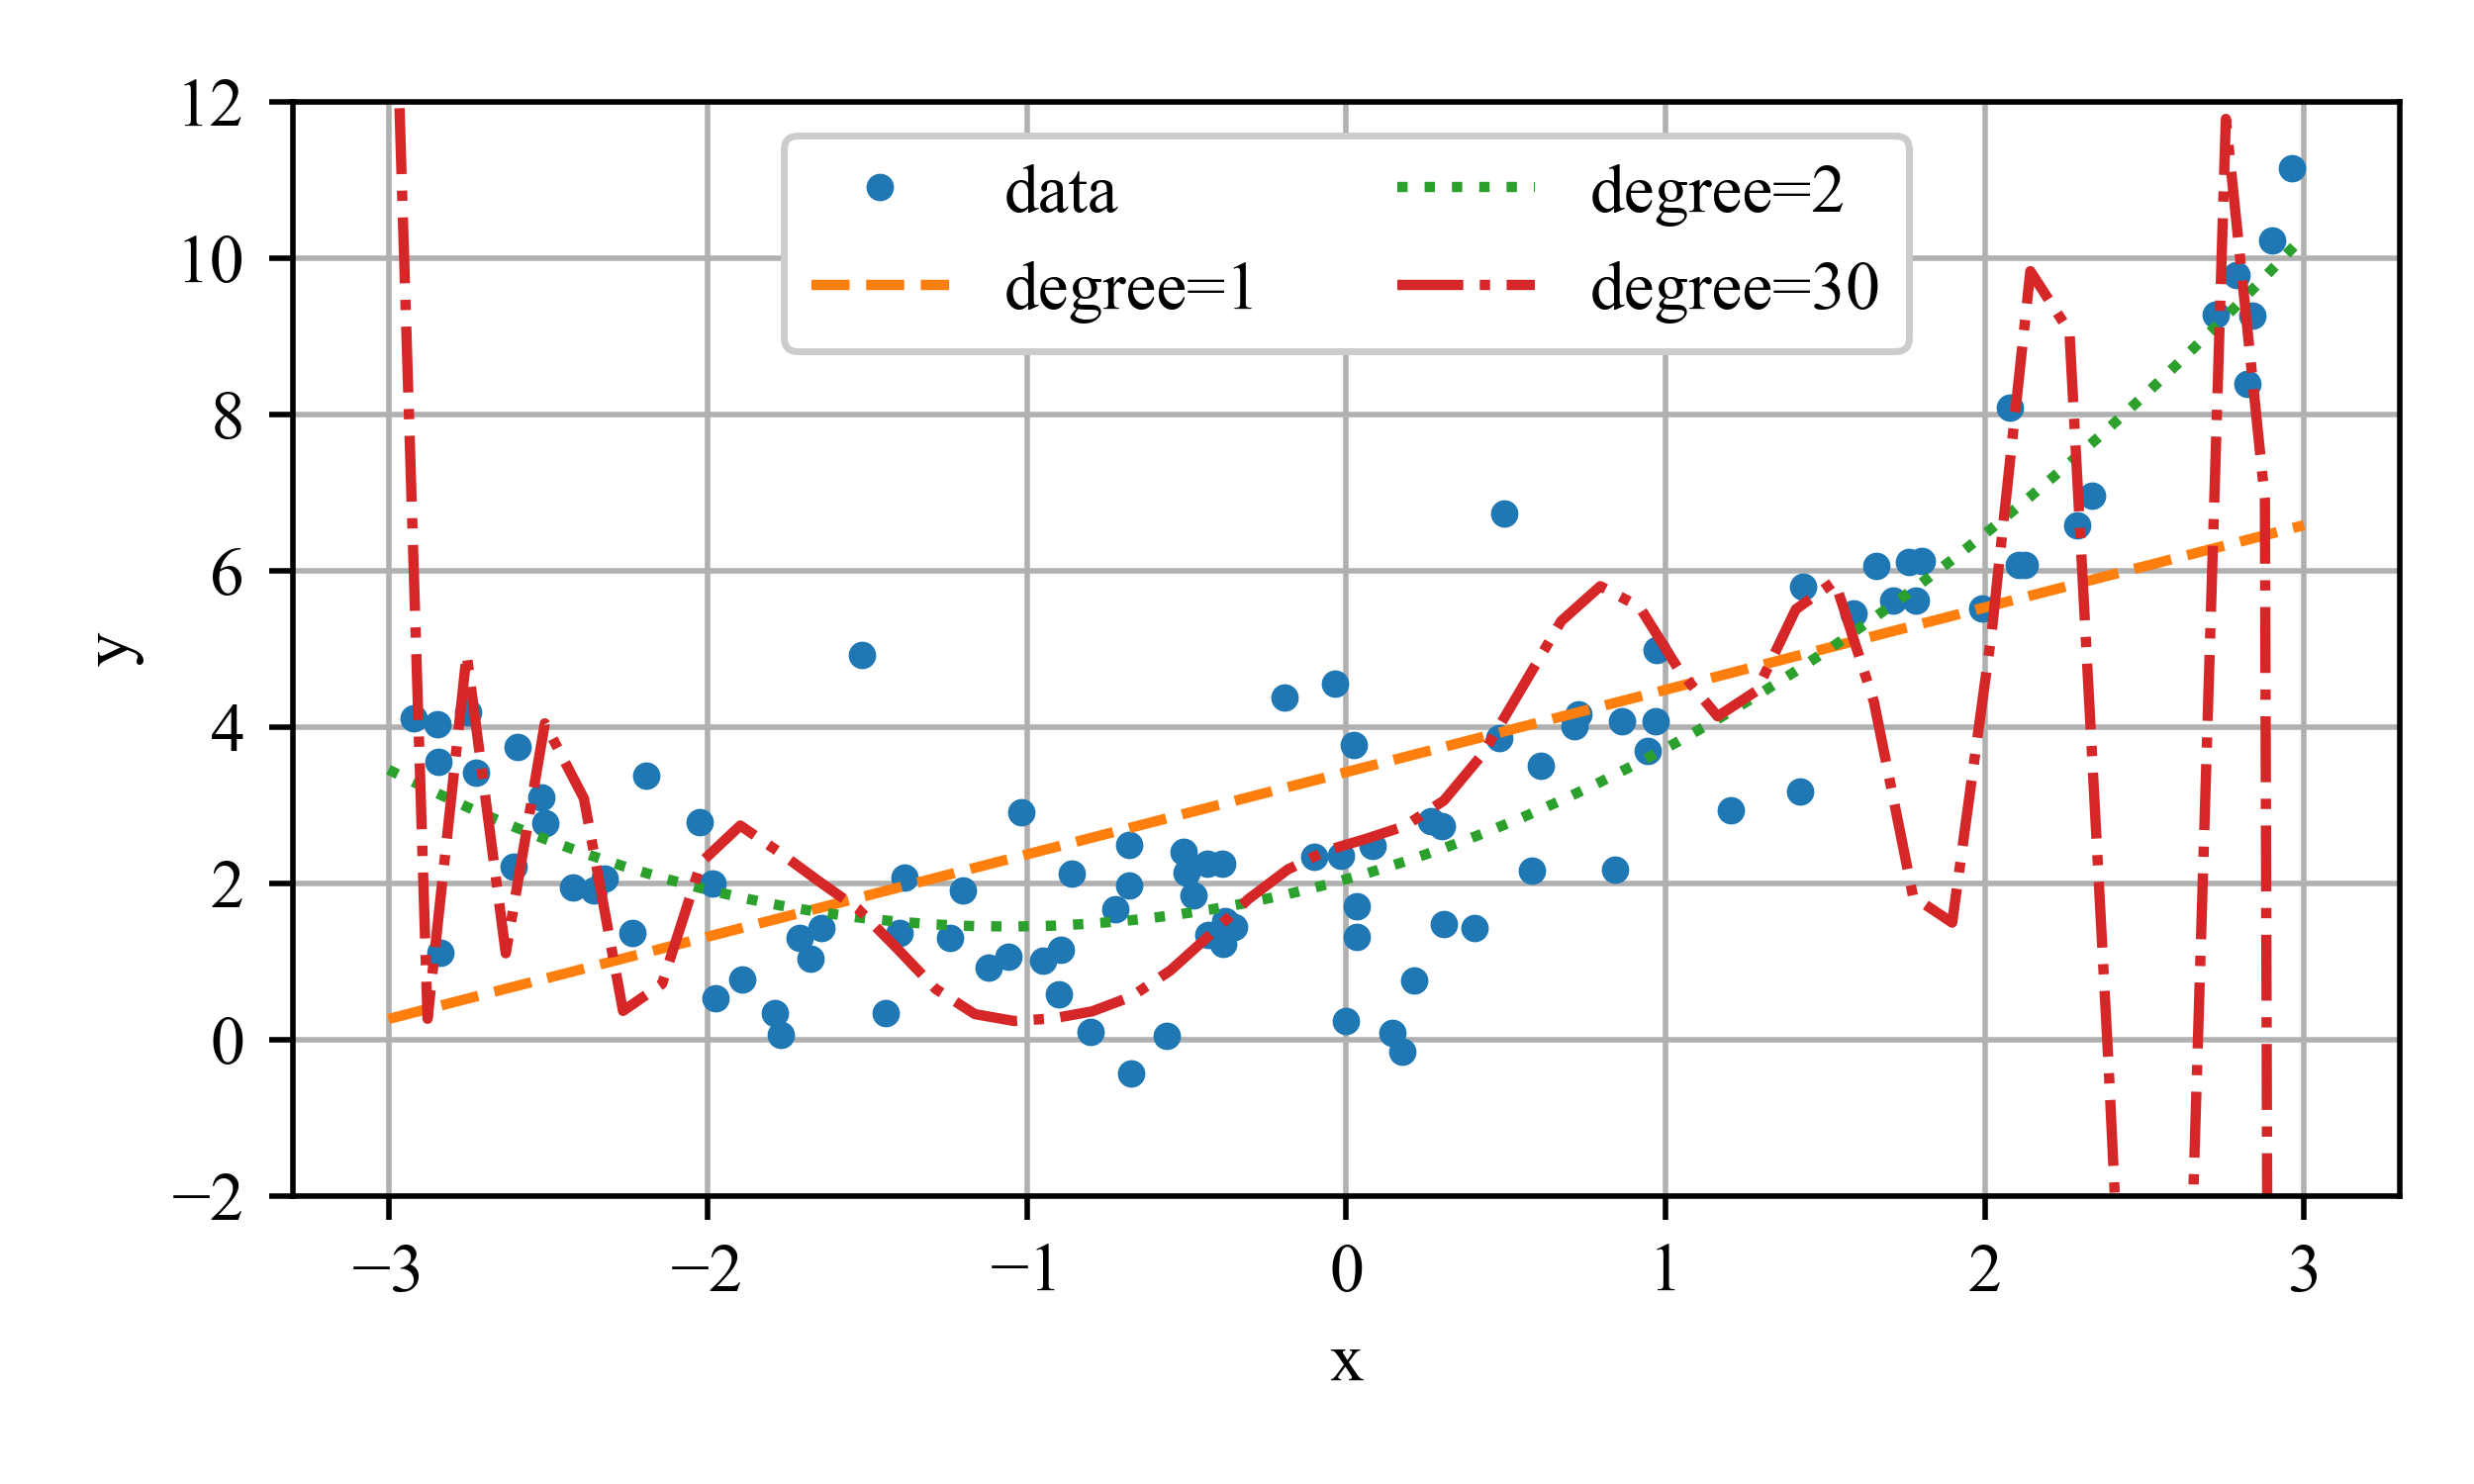
\includegraphics[width=\textwidth]{../figures/overfitting_1.png}
		
		\vspace{0.3em}
		{\small Underfitting, good fit, and overfitting.}
		
	\end{columns}
\end{frame}

%------------------------------------------------

\begin{frame}{Underfitting}
	\begin{columns}
		
		\column{0.48\textwidth}
		
		Characteristics of underfitting:
		
		\vspace{0.5em}
		
		\begin{itemize}
			\item Model is too simple
			\item Cannot capture data complexity
			\item Training and validation errors remain high
		\end{itemize}
		
		\vspace{0.5em}
		
		Learning curves:
		\begin{itemize}
			\item Curves are close together
			\item Errors plateau at high values
		\end{itemize}
		
		\column{0.52\textwidth}
		\centering
		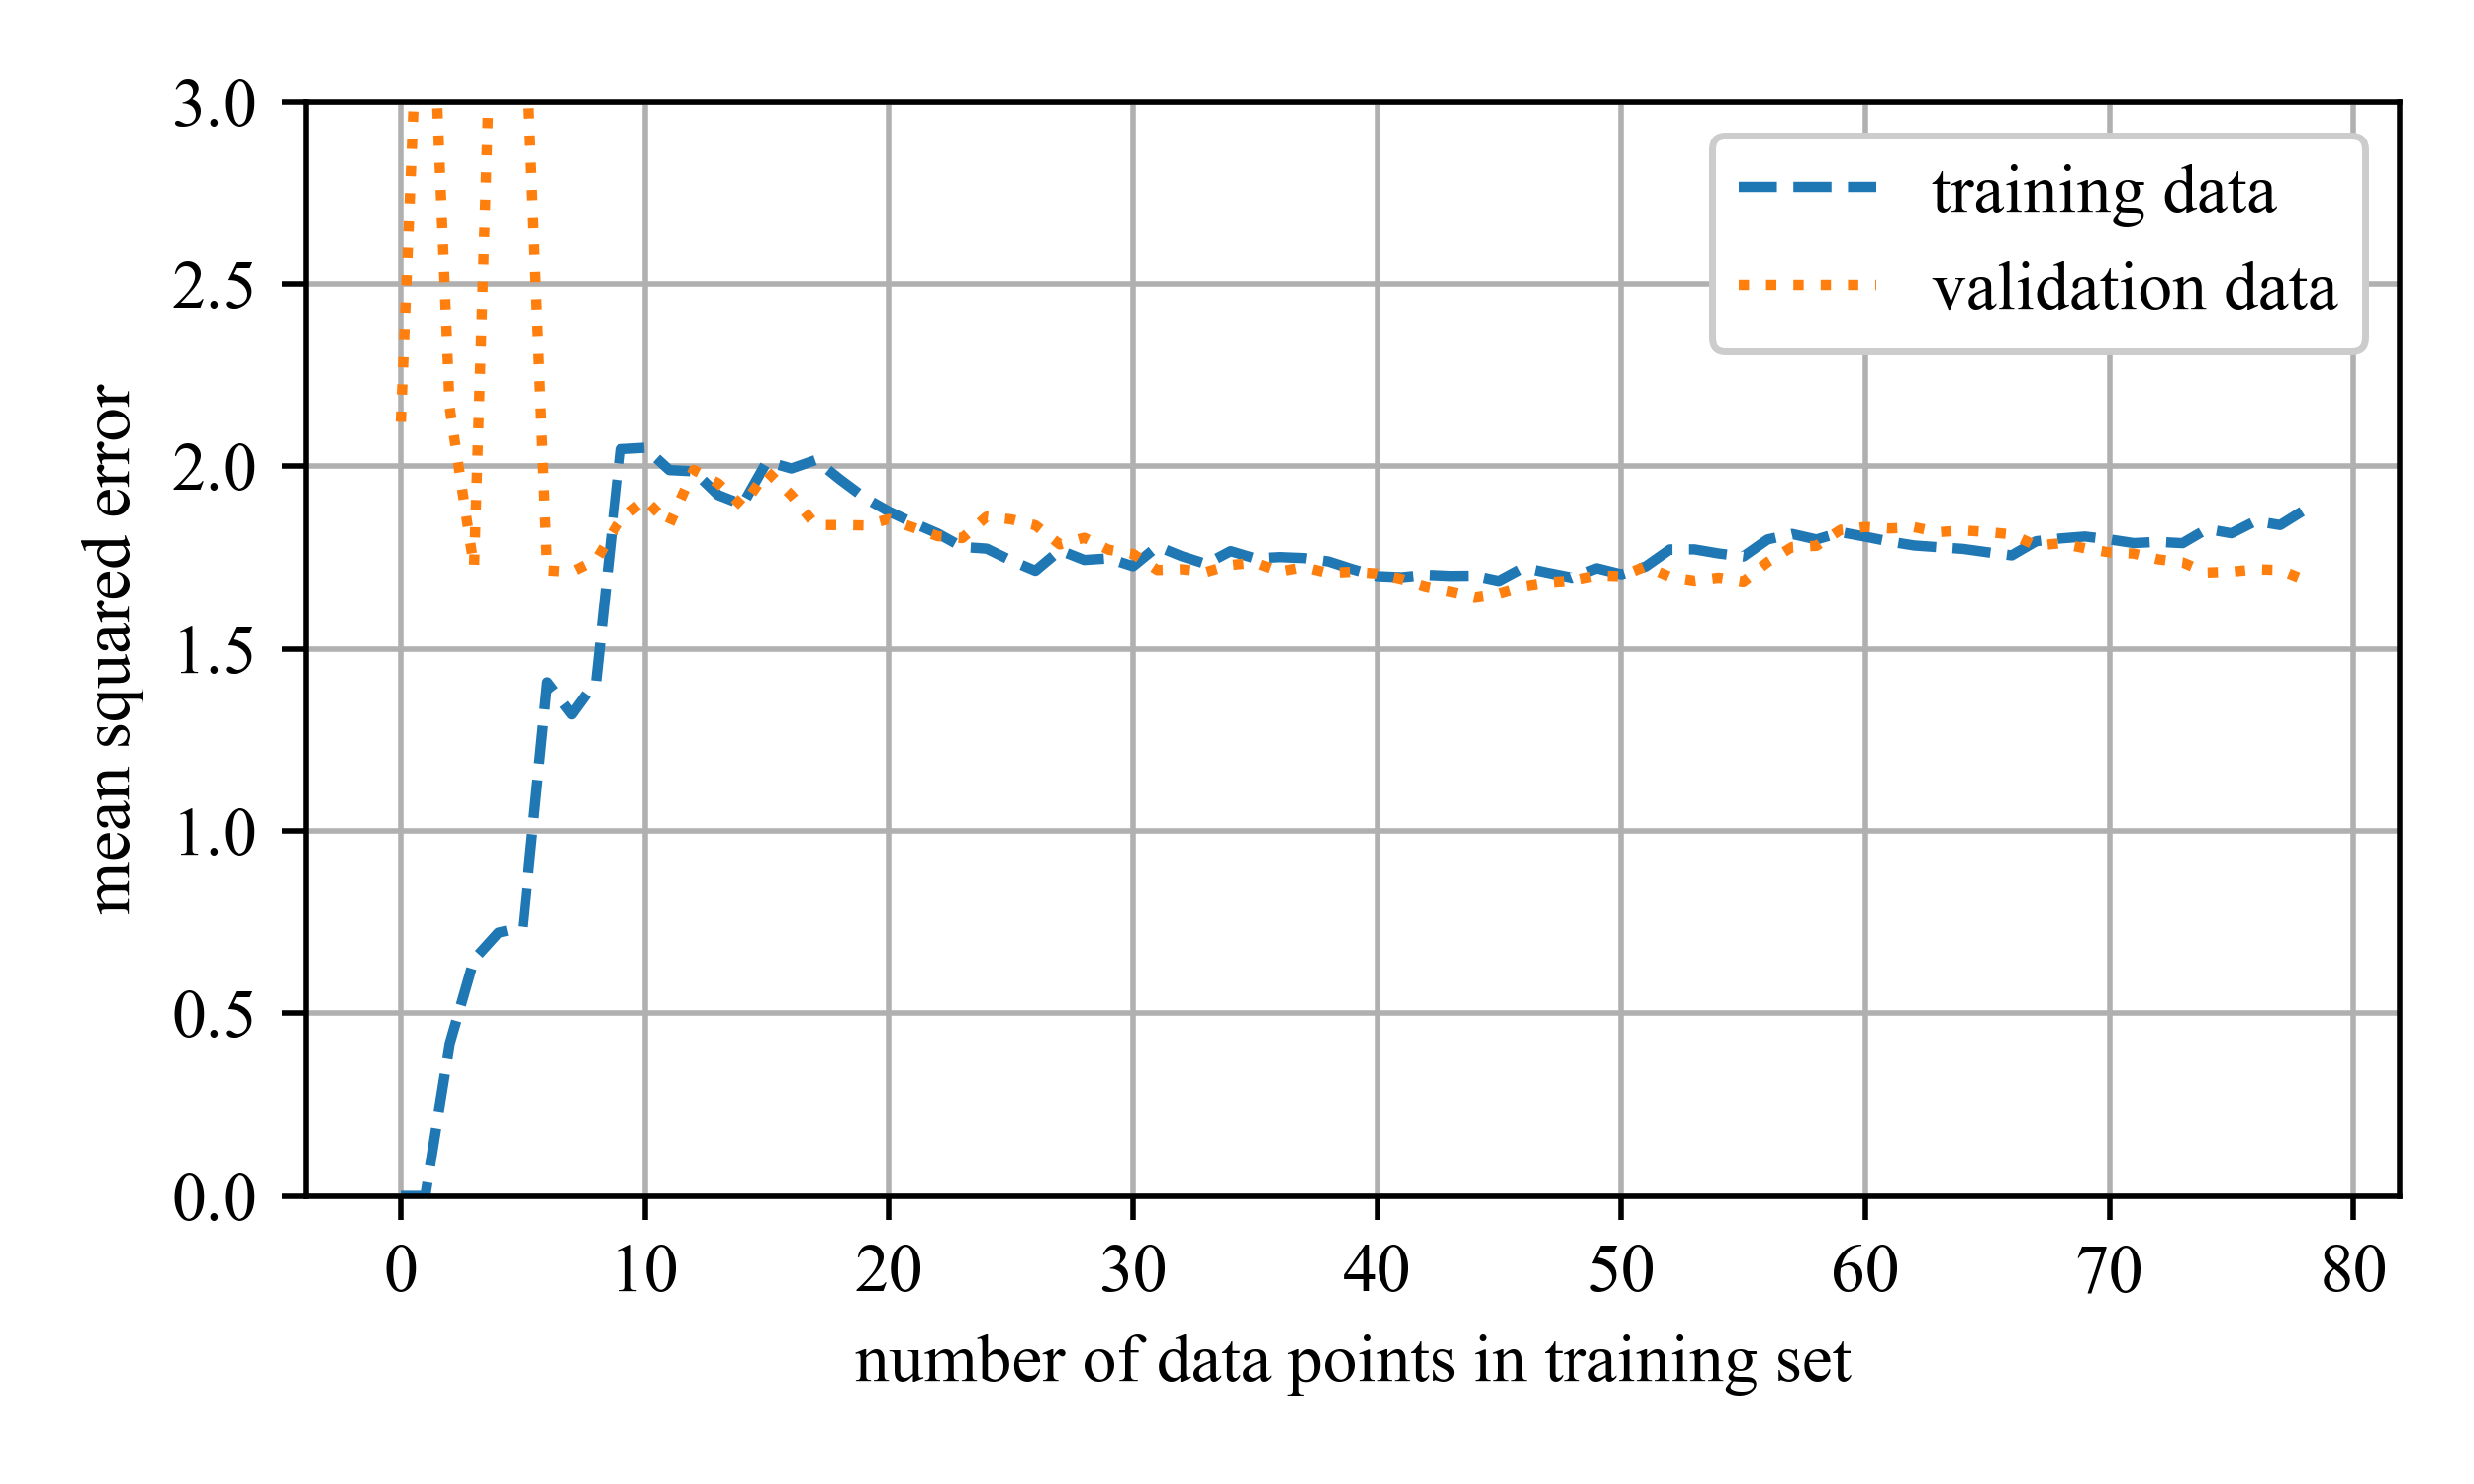
\includegraphics[width=\textwidth]{../figures/overfitting_2.png}
		
		\vspace{0.3em}
		{\small Learning curves for an underfitting model.}
		
	\end{columns}
\end{frame}

%------------------------------------------------

\begin{frame}{Overfitting}
	\begin{columns}
		
		\column{0.48\textwidth}
		
		Characteristics of overfitting:
		
		\vspace{0.5em}
		
		\begin{itemize}
			\item Model is too complex
			\item Fits noise in the training data
			\item Excellent training performance
			\item Poor validation performance
		\end{itemize}
		
		\vspace{0.5em}
		
		Learning curves:
		\begin{itemize}
			\item Large gap between curves
			\item High variance
		\end{itemize}
		
		\column{0.52\textwidth}
		\centering
		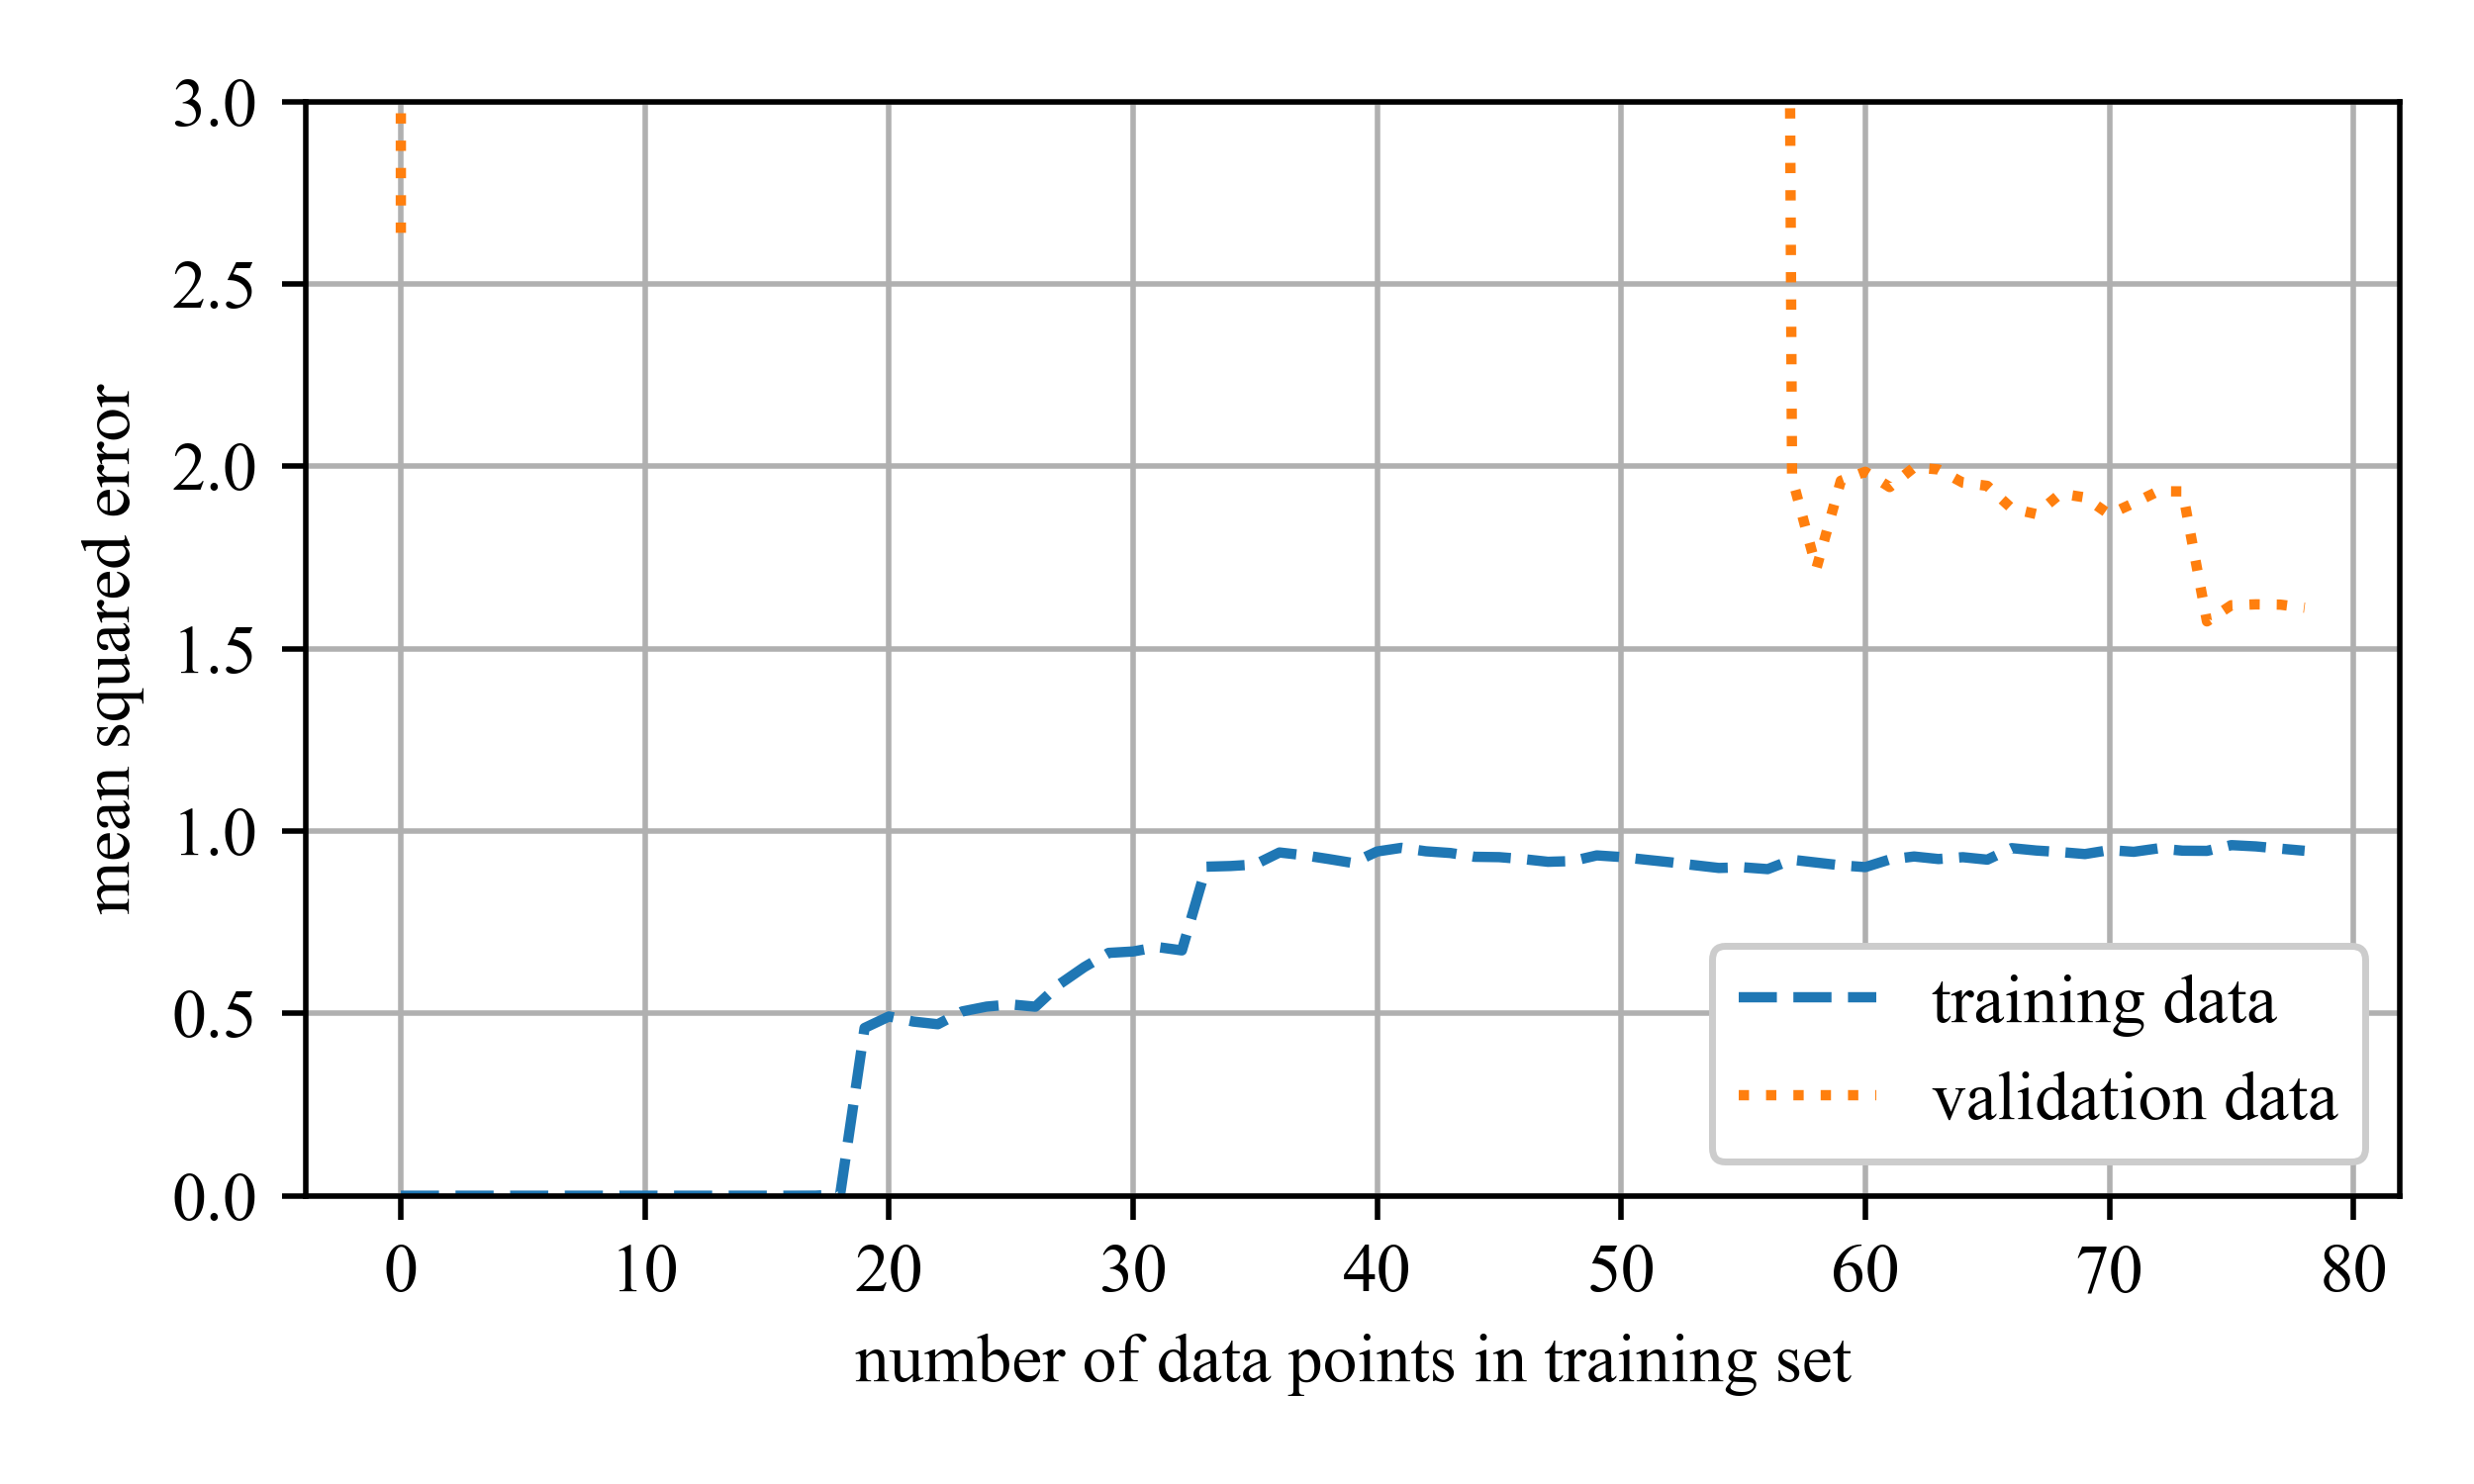
\includegraphics[width=\textwidth]{../figures/overfitting_3.png}
		
		\vspace{0.3em}
		{\small Learning curves for an overfitting model.}
		
	\end{columns}
\end{frame}

%------------------------------------------------

\begin{frame}{Well-Fit Model}
	\begin{columns}
		
		\column{0.48\textwidth}
		
		A good model balances:
		\begin{itemize}
			\item Bias
			\item Variance
		\end{itemize}
		
		\vspace{0.5em}
		
		Characteristics:
		\begin{itemize}
			\item Low training error
			\item Low validation error
			\item Small gap between curves
		\end{itemize}
		
		\vspace{0.5em}
		
		The model generalizes well to unseen data.
		
		\column{0.52\textwidth}
		\centering
		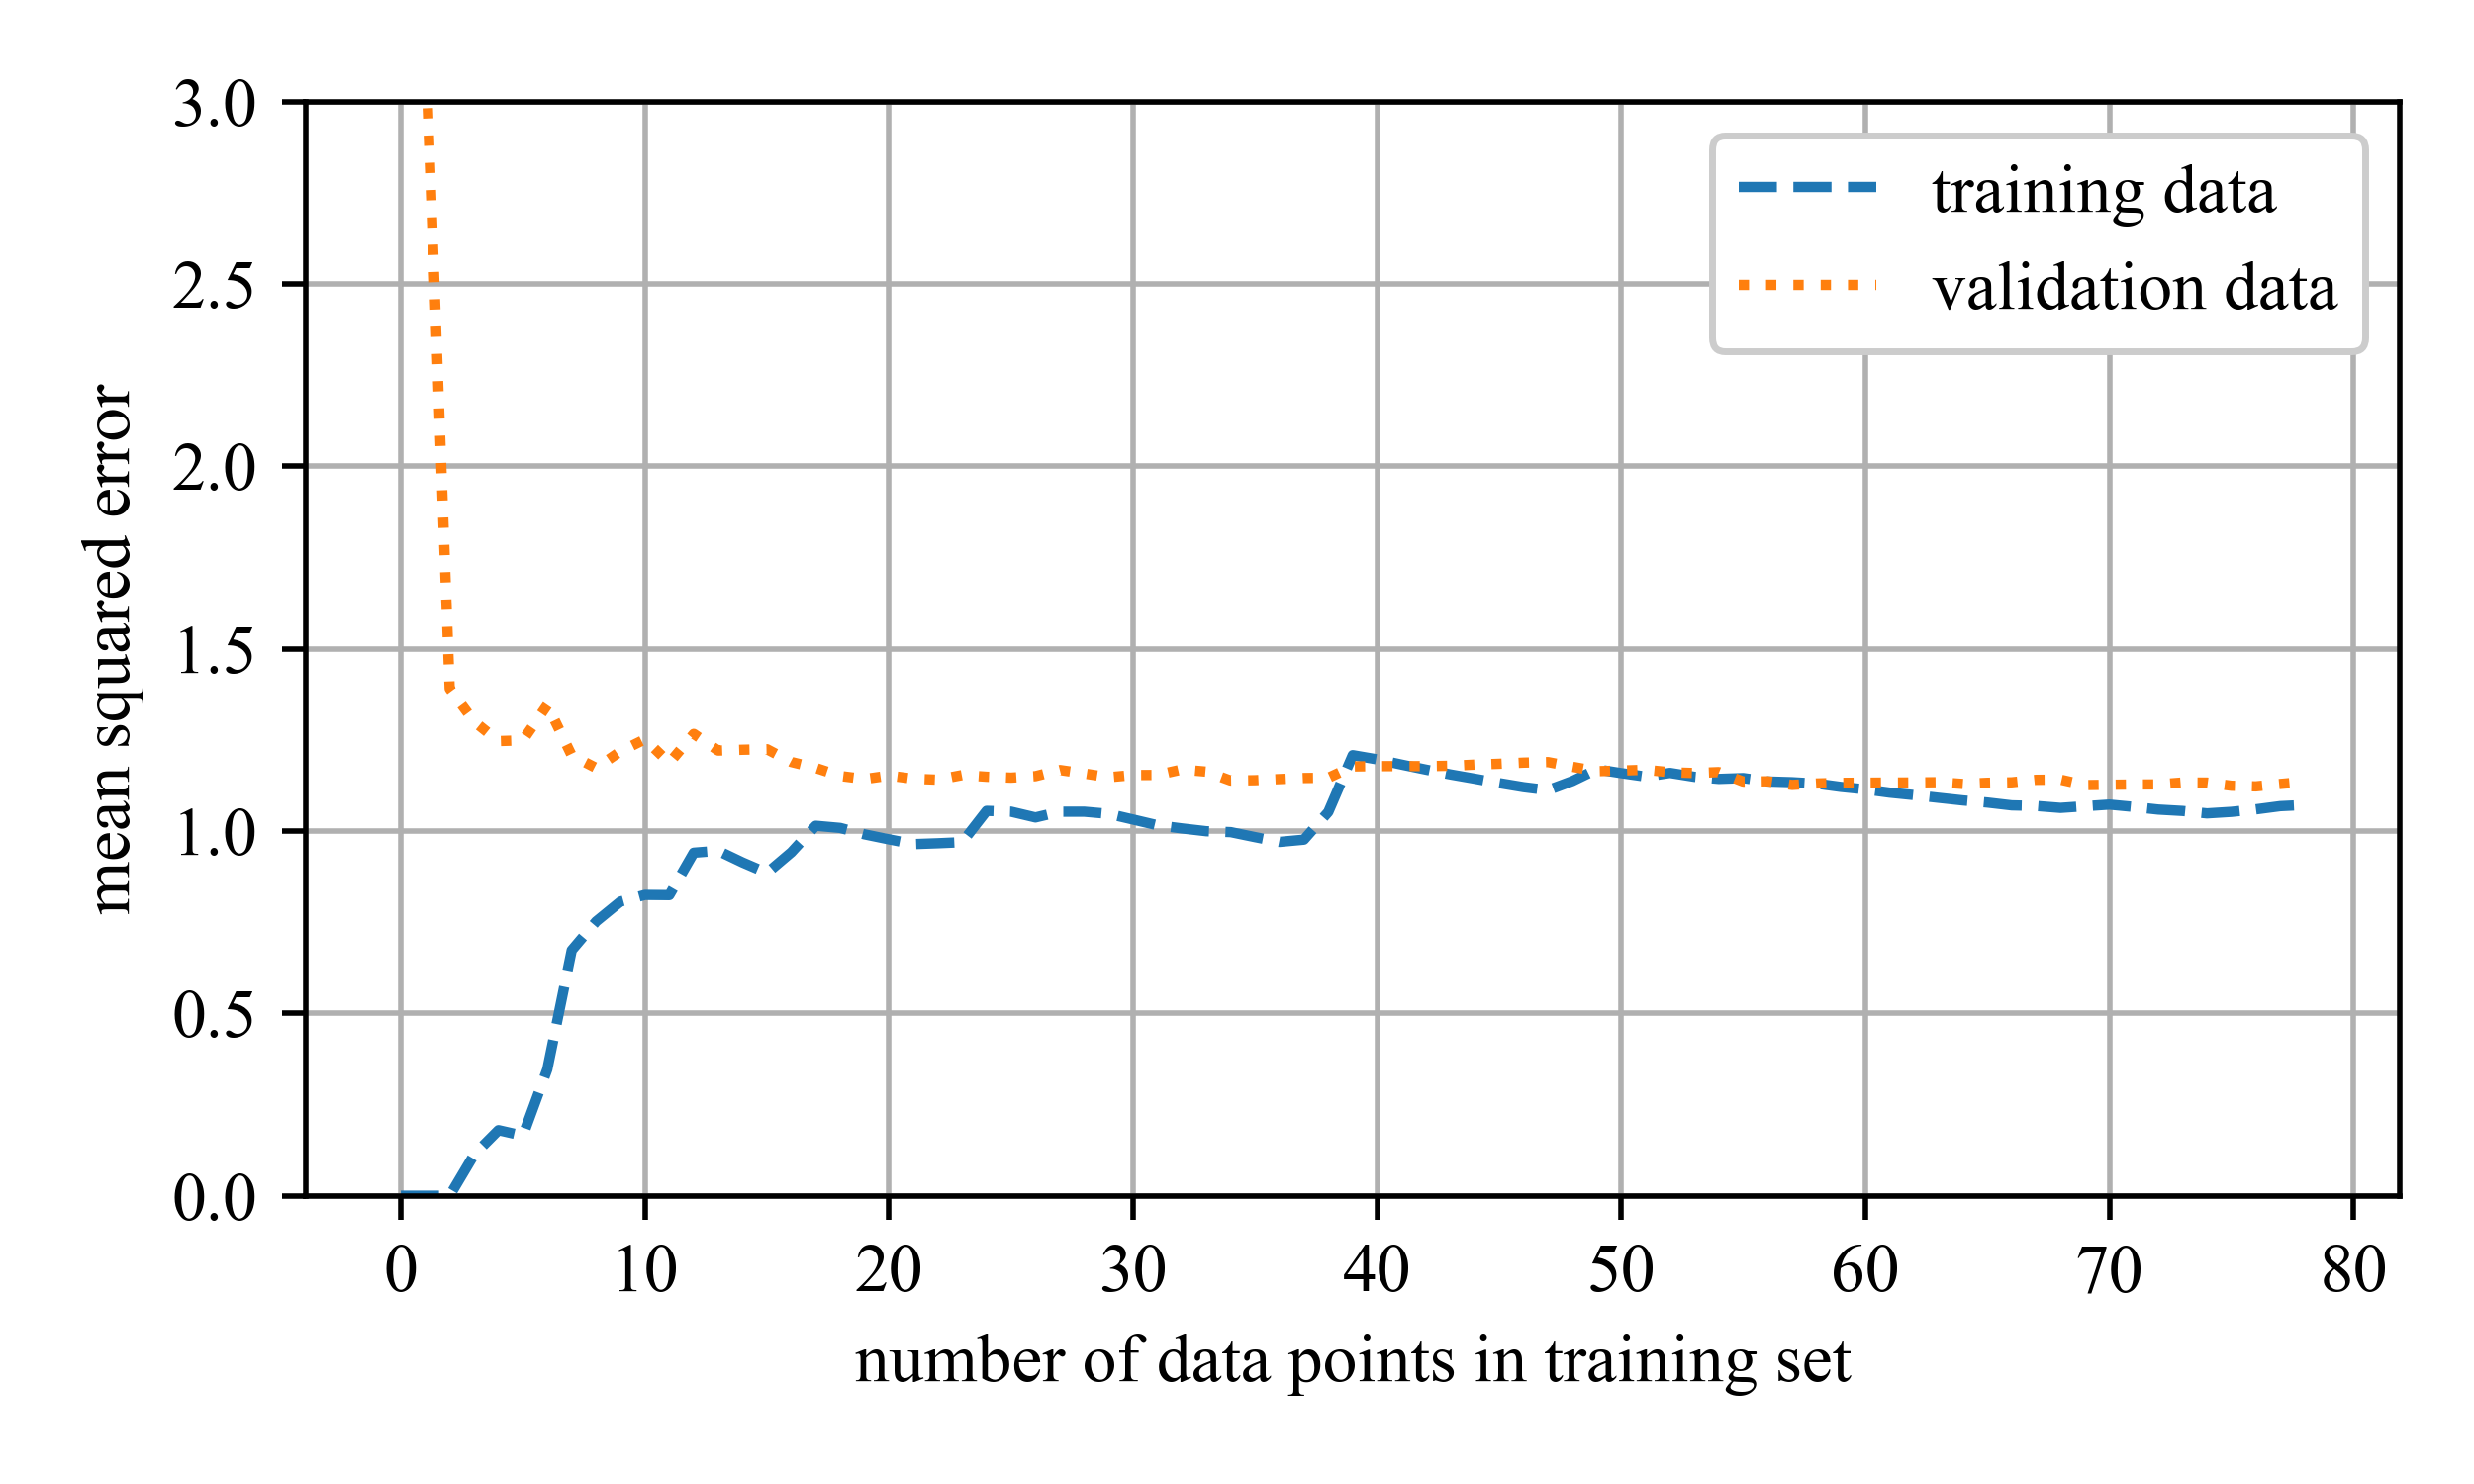
\includegraphics[width=\textwidth]{../figures/overfitting_4.png}
		
		\vspace{0.3em}
		{\small Learning curves for a well-fit model.}
		
	\end{columns}
\end{frame}

%------------------------------------------------

\begin{frame}{Interpreting Learning Curves}
	
	Learning curves compare:
	\[
	\text{Training Error}
	\qquad \text{vs.} \qquad
	\text{Validation Error}
	\]
	
	\vspace{0.7em}
	
	\begin{itemize}
		\item Underfitting:
		\begin{itemize}
			\item Both errors high
			\item Curves close together
		\end{itemize}
		
		\vspace{0.5em}
		
		\item Overfitting:
		\begin{itemize}
			\item Training error low
			\item Validation error much higher
		\end{itemize}
		
		\vspace{0.5em}
		
		\item Good fit:
		\begin{itemize}
			\item Both errors low
			\item Curves converge
		\end{itemize}
	\end{itemize}
	
\end{frame}

%------------------------------------------------

\begin{frame}{Example 2.3: Learning Curves}
	
	\begin{itemize}
		\item Compare learning curves for:
		\begin{itemize}
			\item Linear regression
			\item Polynomial regression
		\end{itemize}
		
		\vspace{0.5em}
		
		\item Plot training and validation errors as the training set grows
		
		\vspace{0.5em}
		
		\item Demonstrates:
		\begin{itemize}
			\item Underfitting
			\item Overfitting
			\item Model generalization
			\item Bias--variance tradeoff
		\end{itemize}
		
		\vspace{0.5em}
		
		\item Shows how model complexity affects performance
	\end{itemize}
	
\end{frame}

%------------------------------------------------
\section{2.8~Regularized Linear Models}

\begin{frame}{Regularized Linear Models}
	
	Overfitting can be reduced through:
	
	\[
	\textbf{Regularization}
	\]
	
	\vspace{0.5em}
	
	Idea:
	\begin{itemize}
		\item Constrain model complexity
		\item Prevent fitting noise in the data
		\item Improve generalization
	\end{itemize}
	
	\vspace{0.5em}
	
	For polynomial models:
	\begin{itemize}
		\item Use a lower polynomial degree
	\end{itemize}
	
	\vspace{0.5em}
	
	For linear models:
	\begin{itemize}
		\item Penalize large coefficient values
	\end{itemize}
	
\end{frame}

%------------------------------------------------


\begin{frame}{Ridge Regression}
	\begin{columns}
		
		\column{0.48\textwidth}
		
		Ridge Regression adds a penalty term to the cost function:
		
		\[
		J(\theta)
		=
		\text{MSE}(\theta)
		+
		\alpha
		\frac{1}{2}
		\sum_{i=1}^{n}\theta_i^2
		\]
		
		\vspace{0.5em}
		
		\begin{itemize}
			\item $\alpha$: regularization strength
			\item Large $\alpha$ $\rightarrow$ smaller weights
			\item Reduces overfitting
		\end{itemize}
		
		\vspace{0.5em}
		
		\begin{exampleblock}{Note}
			The bias term $\theta_0$ is not regularized.
		\end{exampleblock}
		
		\column{0.52\textwidth}
		\centering
		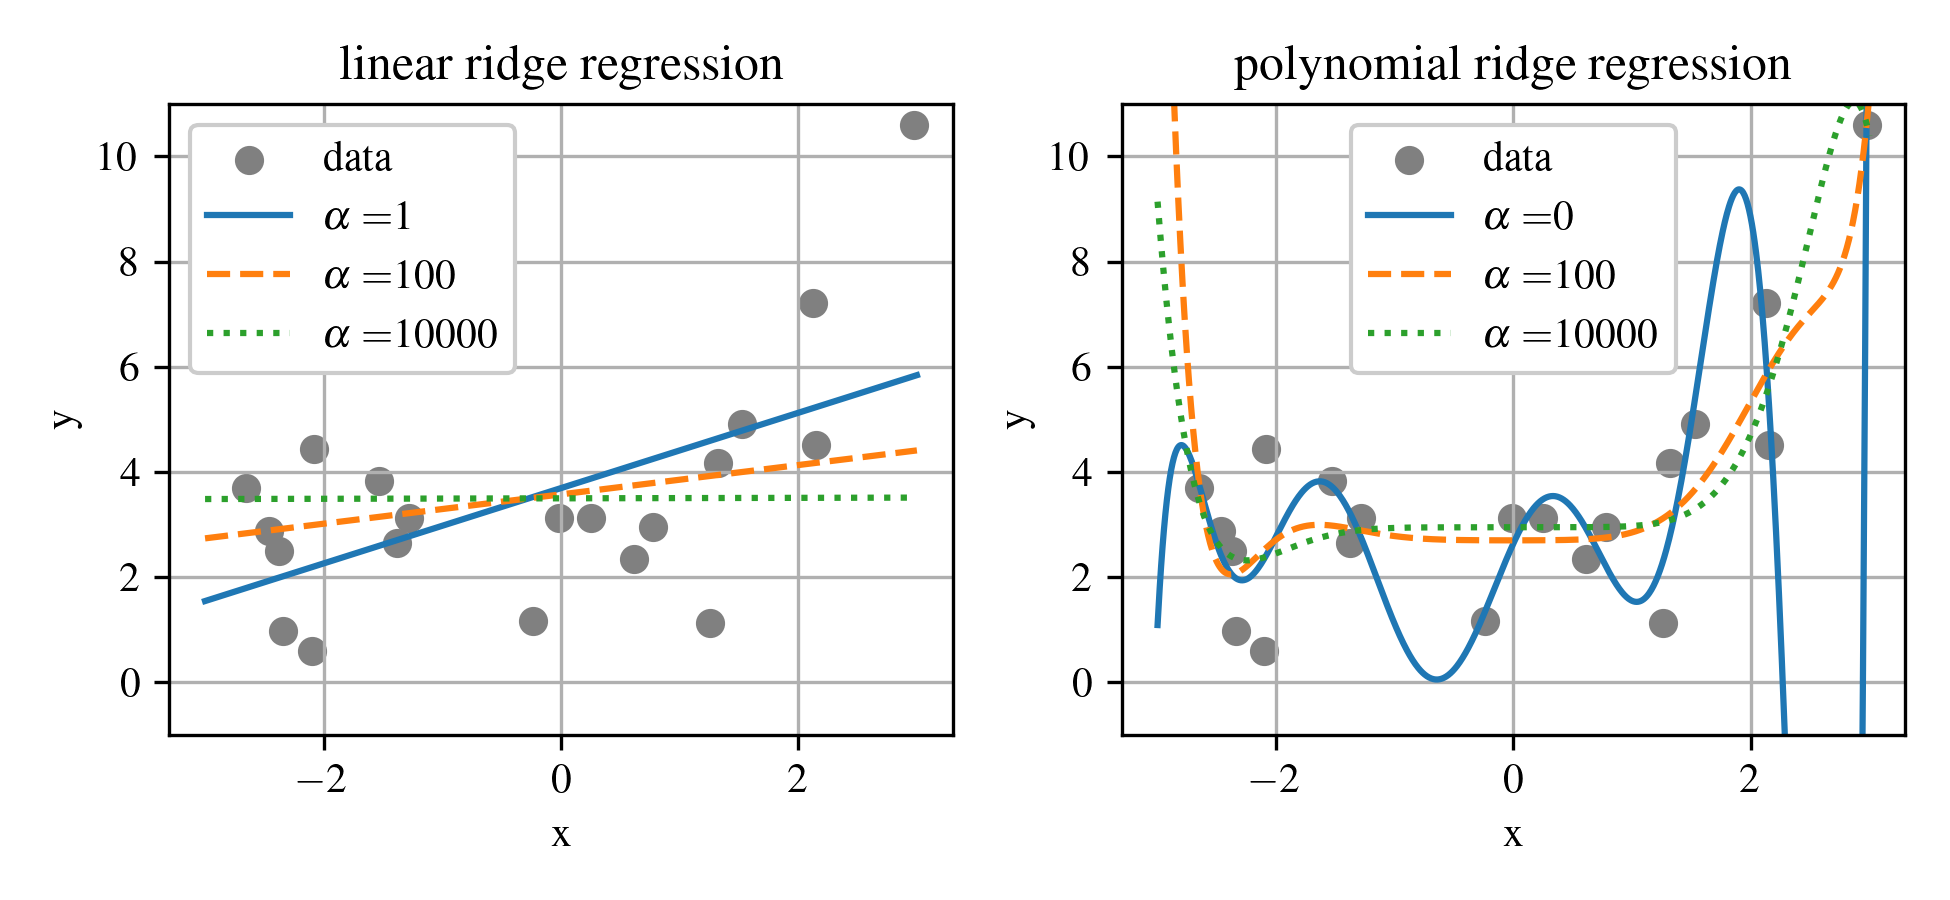
\includegraphics[width=\textwidth]{../figures/ridge_regression.png}
		
		\vspace{0.3em}
		{\small Ridge regression with different $\alpha$ values.}
		
	\end{columns}
\end{frame}

%------------------------------------------------

\begin{frame}{Example 2.4: Ridge Regression}
	
	\begin{itemize}
		\item Apply Ridge Regression to a high-degree polynomial model
		\item Add regularization to reduce overfitting
		\item Use a pipeline with:
		\begin{itemize}
			\item \texttt{PolynomialFeatures}
			\item \texttt{StandardScaler}
			\item \texttt{Ridge}
		\end{itemize}
		
		\vspace{0.5em}
		
		\item Demonstrates:
		\begin{itemize}
			\item Smoother predictions
			\item Reduced variance
			\item Improved model stability
		\end{itemize}
		
		\vspace{0.5em}
		
		\item Compare different values of $\alpha$
	\end{itemize}
	
\end{frame}

%------------------------------------------------
\section{2.9~Early Stopping}

\begin{frame}{Early Stopping}
	\begin{columns}
		
		\column{0.48\textwidth}
		
		Early stopping is a form of regularization for iterative learning methods.
		
		\vspace{0.5em}
		
		Idea:
		\begin{itemize}
			\item Monitor validation error during training
			\item Stop training when validation error begins increasing
		\end{itemize}
		
		\vspace{0.5em}
		
		Benefits:
		\begin{itemize}
			\item Prevents overfitting
			\item Improves generalization
			\item Simple and computationally inexpensive
		\end{itemize}
		
		\vspace{0.5em}
		
		\column{0.52\textwidth}
		\begin{exampleblock}{Key Idea}
			Stop training at the minimum validation error.
		\end{exampleblock}

		\vspace{1.5em}
		
		\centering
		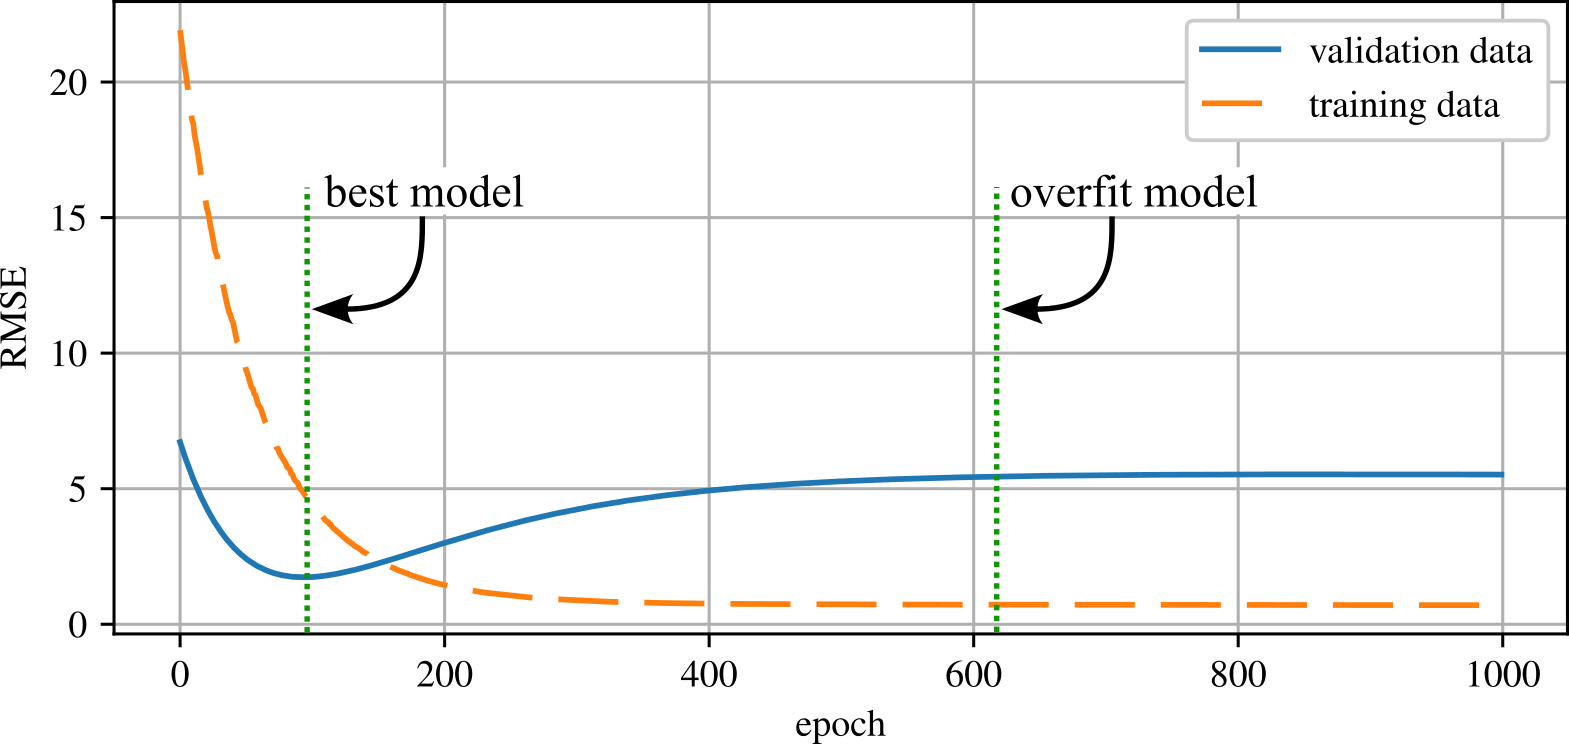
\includegraphics[width=\textwidth]{../figures/early_stopping.png}
		
		\vspace{0.3em}
		{\small Early stopping prevents overfitting.}
		
	\end{columns}
\end{frame}

%------------------------------------------------

\begin{frame}{Example 2.5: Early Stopping}
	
	\begin{itemize}
		\item Train a high-degree polynomial model using:
		\begin{itemize}
			\item Stochastic Gradient Descent
		\end{itemize}
		
		\vspace{0.5em}
		
		\item Track:
		\begin{itemize}
			\item Training error
			\item Validation error
		\end{itemize}
		
		\vspace{0.5em}
		
		\item Demonstrates:
		\begin{itemize}
			\item How overfitting develops during training
			\item How validation error identifies the optimal stopping point
			\item Improved generalization through early stopping
		\end{itemize}
		
		\vspace{0.5em}
		
		\item Training halts once validation performance begins degrading
	\end{itemize}
	
\end{frame}








































\end{document}




